\documentclass{subfiles}

\begin{document}

\subsection{Absorption und Emission}
    Im groben Bild stellen wir uns den Aufbau eines Atoms als einen Kern mit Elektronen vor, welche sich auf Kreisbahnen um den Kern bewegen. Letztere bezeichnen wir als \emph{Elektronenhülle}, welche nachfolgend Untersuchungsgegenstand sein wird. 

    \begin{figure}[H]
        \centering
        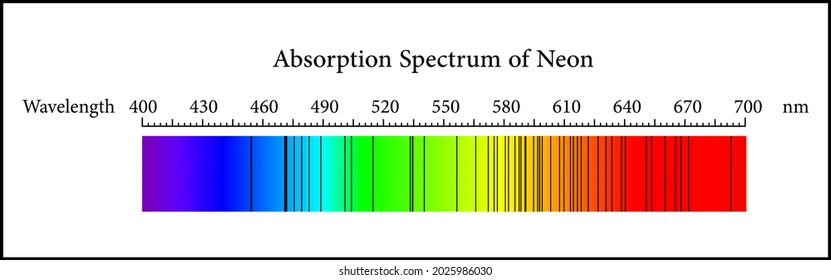
\includegraphics[width=5cm]{Bilddateien/AbsorbtionsspektrumNeon.png}
        \caption{Emissionsspektrum am Beispiel von Neon aus \cite{sutterstock:AbsorbtionNeon}.}
    \end{figure}

    \begin{figure}[H]
        \centering
        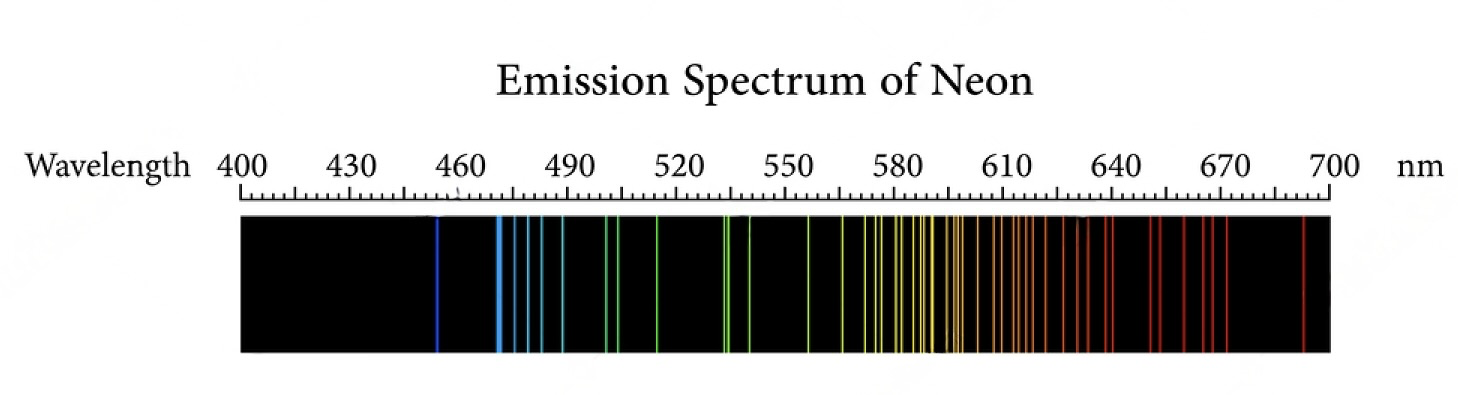
\includegraphics[width=5cm]{Bilddateien/EmissionsspektrumNeon-transformed.png}
        \caption{Absorbtionsspektrum am Beispiel von Neon aus \cite{sutterstock:EmissionNeon}.}
    \end{figure}
    Diese Spektren stellen sich als \emph{charakteristisch} für Atome heraus. Als Beispiel gilt hier die \emph{Balmer-Serie} [$\to$ AP4], welche sich durch die Formel
    \[\tilde\nu = \lambda^{-1} = R_H\cdot\nbra{\frac{1}{4} - \frac{1}{n^2}},\quad n\in\N_{>2},\]
    in \emph{normierter Form} beschreiben lässt. Dabei bezeichnet $R_H$ die \emph{Rydberg-Konstante} mit $R_H = 1.097\cdot 10^7\si{\per\meter}$. Multipliziert mit $c_0$ erhalten wir die \emph{Rydberg-Frequenz} $\nu_R = \tilde\nu\cdot c_0$. Die Betrachtung $n\to\infty$ ergibt das \emph{Serien-Grenzkontinuum} $\nu = 1/4\cdot R_H\cdot c_0$. In diesem Bereich weist das Spektrum keine Linien mehr vor, sondern ist kontinuierlich. Bei Wasserstoff stellt sich heraus, daß es noch weitere Serien gibt; Eine davon ist die \emph{Rydberg-Serie} mit
    \[\nu = R_H\cdot c_0\cdot \nbra{\frac{1}{k^2} - \frac{1}{n^2}},\quad n\in\N_{>1},\; n>k.\] 
    
    
    \begin{Aufgabe}
        \nr{} Erkläre, warum die Spektren zueinander komplementär erscheinen. Handelt es sich dabei um eine Phänomenologie, oder lässt sich dies auch theoretisch begründen?
    \end{Aufgabe}
\end{document}